\documentclass[10pt]{article}
\usepackage[latin1]{inputenc}
\usepackage{tikz}
\usepackage{caption}
\usepackage[margin=0.25in]{geometry}
\usetikzlibrary{shapes,arrows}
\newcommand*{\h}{\hspace{5pt}}% for indentation
\newcommand*{\hh}{\h\h}% double indentation
\begin{document}
\begin{center}
  \captionof{figure}{Flowchart of Sulphur Clock Reaction}
  \footnotesize
  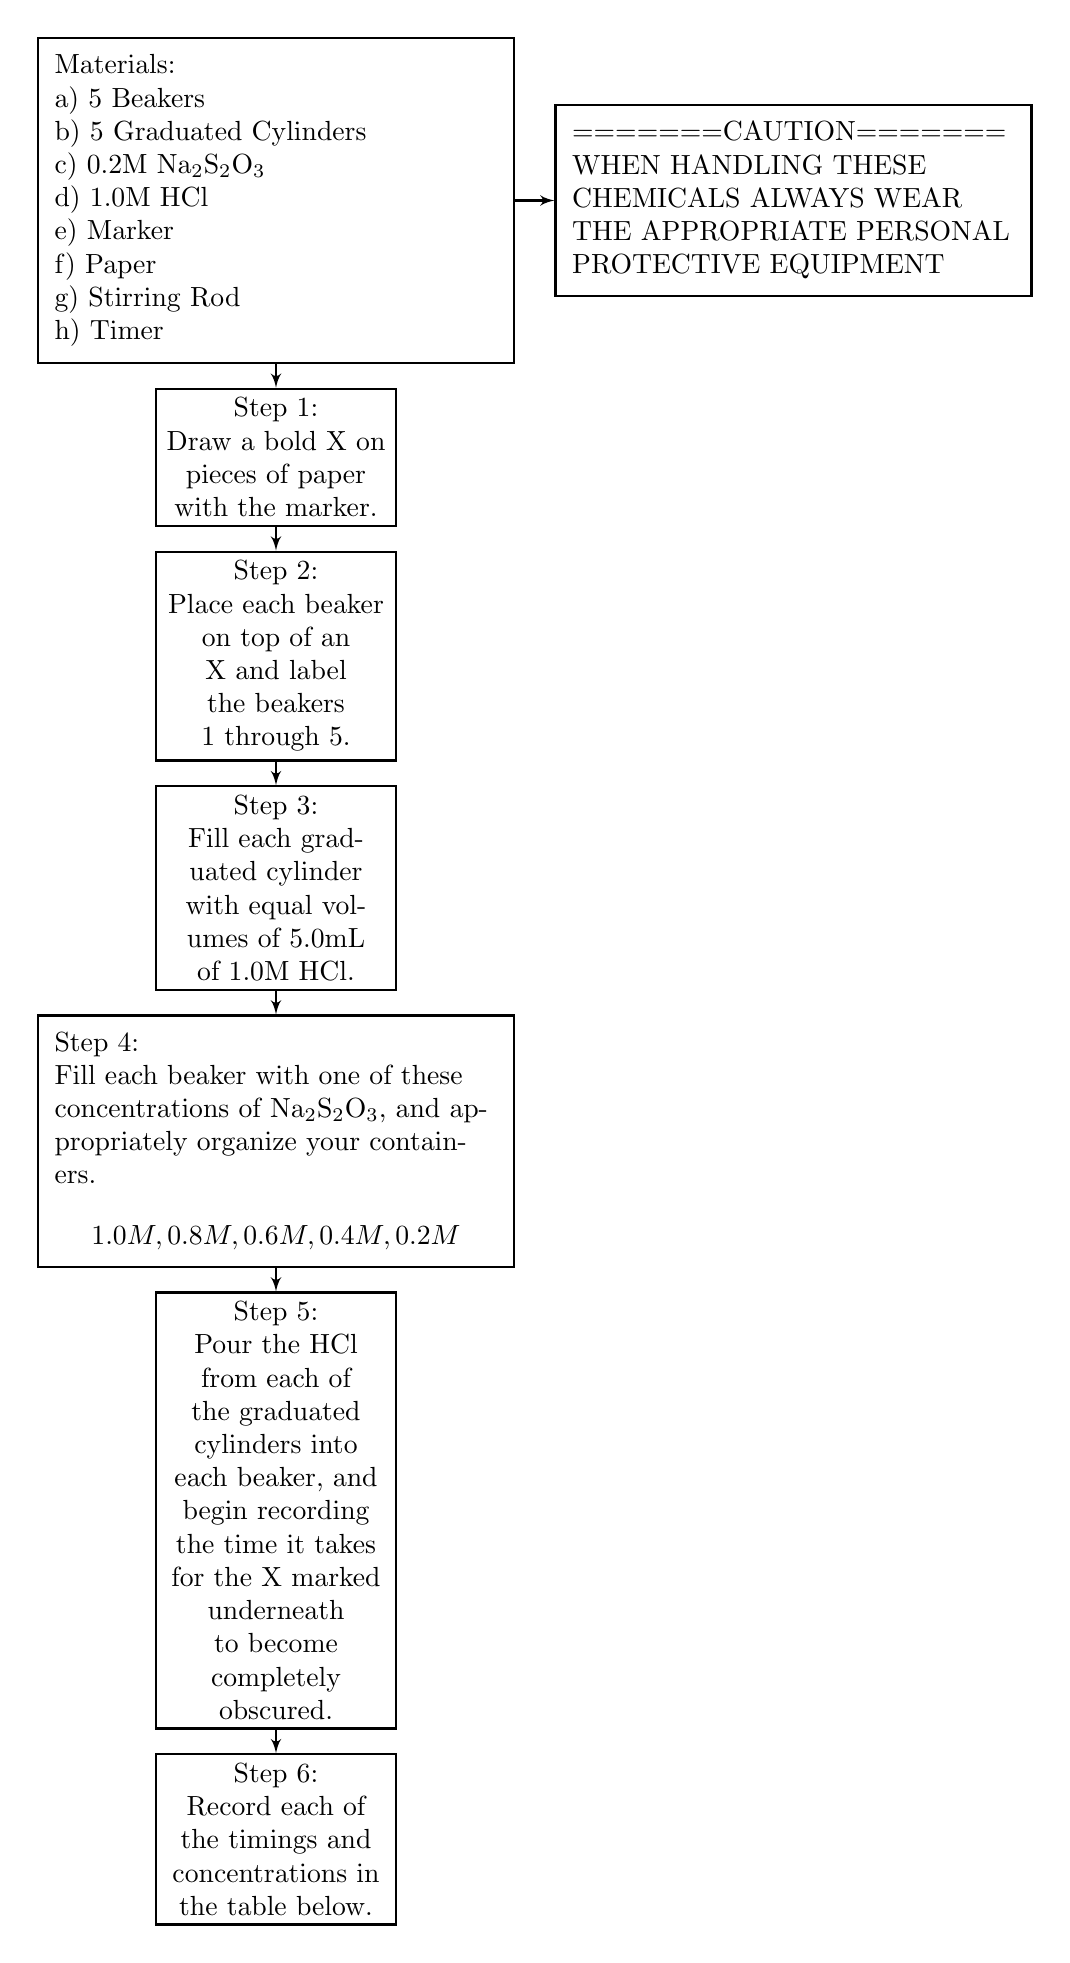
\begin{tikzpicture}[auto,
    %decision/.style={diamond, draw=black, thick, fill=white,
    %text width=8em, text badly centered,
    %inner sep=1pt, font=\sffamily\small},
    block_center/.style ={rectangle, draw=black, thick, fill=white, text width=8em, text centered,
      minimum height=4em},
    block_left/.style ={rectangle, draw=black, thick, fill=white,
      text width=16em, text ragged, minimum height=4em, inner sep=6pt},
    block_noborder/.style ={rectangle, draw=none, thick, fill=none,
      text width=18em, text centered, minimum height=1em},
    block_assign/.style ={rectangle, draw=black, thick, fill=white,
      text width=18em, text ragged, minimum height=3em, inner sep=6pt},
    block_lost/.style ={rectangle, draw=black, thick, fill=white,
      text width=16em, text ragged, minimum height=3em, inner sep=6pt},
      line/.style ={draw, thick, -latex', shorten >=0pt}]
    % outlining the flowchart using the PGF/TikZ matrix funtion
    \matrix [column sep=5mm,row sep=3mm] {
      % enrollment - row 1
		\node [block_left] (materials) {
		Materials: \\
        	a) 5 Beakers \\
        	b) 5 Graduated Cylinders \\
	        c) 0.2M Na\textsubscript{2}S\textsubscript{2}O\textsubscript{3}\\
        	d) 1.0M HCl \\
        	e) Marker \\
        	f) Paper \\
        	g) Stirring Rod\\
        	h) Timer};
		& \node [block_left] (caution) {
		=======CAUTION======= \\
        	WHEN HANDLING THESE CHEMICALS ALWAYS WEAR THE APPROPRIATE PERSONAL PROTECTIVE EQUIPMENT}; \\
      % enrollment - row 2
		\node [block_center] (step1) {
		Step 1: \\
		Draw a bold X on  pieces of paper with the marker.};\\
		\node [block_center] (step2) {
		Step 2: \\
		Place each beaker on top of an X and label the beakers 1 through 5.};\\
		\node [block_center] (step3) {
		Step 3: \\
		Fill each graduated cylinder with equal volumes of 5.0mL of 1.0M HCl.};\\
		\node [block_left] (step4) {
		Step 4: \\
		Fill each beaker with one of these concentrations of Na\textsubscript{2}S\textsubscript{2}O\textsubscript{3}, and appropriately organize your containers.\\
		\[1.0M, 0.8M, 0.6M, 0.4M, 0.2M\]};\\
		\node [block_center] (step5) {
		Step 5: \\
		Pour the HCl from each of the graduated cylinders into each beaker, and begin recording the time it takes for the X marked underneath to become completely obscured. };\\
		\node [block_center] (step6) {
		Step 6: \\
		Record each of the timings and concentrations in the table below.};\\
	};% end matrix
    % connecting nodes with paths
    \begin{scope}[every path/.style=line]
      % paths for enrollemnt rows
		\path (materials) -- (caution);	
		\path (materials) -- (step1);
		\path (step1) -- (step2);
		\path (step2) -- (step3);
		\path (step3) -- (step4);
		\path (step4) -- (step5);
		\path (step5) -- (step6);
    \end{scope}
  \end{tikzpicture}
\end{center}
\begin{table}[h!]
\centering
\caption{Chart}
\label{my-label}
\begin{tabular}{c|l|l|l|l}
Beaker & \multicolumn{1}{c|}{2.0M of Na\textsubscript{2}S\textsubscript{2}O\textsubscript{3} (mL)} & \multicolumn{1}{c|}{H\textsubscript{2}O (mL)} & \multicolumn{1}{c|}{{[}Na\textsubscript{2}S\textsubscript{2}O\textsubscript{3}{]} moles/L} & \multicolumn{1}{c}{Time (sec)} \\ \hline
A      &                                           &                               &                                            &                                \\
B      &                                           &                               &                                            &                                \\
C      &                                           &                               &                                            &                                \\
D      &                                           &                               &                                            &                                \\
E      &                                           &                               &                                            &                               
\end{tabular}
\end{table}
Manufactured by Kunal Chandan
\end{document}